\documentclass[]{article}
\usepackage{lmodern}
\usepackage{amssymb,amsmath}
\usepackage{ifxetex,ifluatex}
\usepackage{fixltx2e} % provides \textsubscript
\ifnum 0\ifxetex 1\fi\ifluatex 1\fi=0 % if pdftex
  \usepackage[T1]{fontenc}
  \usepackage[utf8]{inputenc}
\else % if luatex or xelatex
  \ifxetex
    \usepackage{mathspec}
  \else
    \usepackage{fontspec}
  \fi
  \defaultfontfeatures{Ligatures=TeX,Scale=MatchLowercase}
\fi
% use upquote if available, for straight quotes in verbatim environments
\IfFileExists{upquote.sty}{\usepackage{upquote}}{}
% use microtype if available
\IfFileExists{microtype.sty}{%
\usepackage[]{microtype}
\UseMicrotypeSet[protrusion]{basicmath} % disable protrusion for tt fonts
}{}
\PassOptionsToPackage{hyphens}{url} % url is loaded by hyperref
\usepackage[unicode=true]{hyperref}
\hypersetup{
            pdfborder={0 0 0},
            breaklinks=true}
\urlstyle{same}  % don't use monospace font for urls
\IfFileExists{parskip.sty}{%
\usepackage{parskip}
}{% else
\setlength{\parindent}{0pt}
\setlength{\parskip}{6pt plus 2pt minus 1pt}
}
\setlength{\emergencystretch}{3em}  % prevent overfull lines
\providecommand{\tightlist}{%
  \setlength{\itemsep}{0pt}\setlength{\parskip}{0pt}}
\setcounter{secnumdepth}{0}
% Redefines (sub)paragraphs to behave more like sections
\ifx\paragraph\undefined\else
\let\oldparagraph\paragraph
\renewcommand{\paragraph}[1]{\oldparagraph{#1}\mbox{}}
\fi
\ifx\subparagraph\undefined\else
\let\oldsubparagraph\subparagraph
\renewcommand{\subparagraph}[1]{\oldsubparagraph{#1}\mbox{}}
\fi

% set default figure placement to htbp
\makeatletter
\def\fps@figure{htbp}
\makeatother

\usepackage{graphicx}

\date{}

\begin{document}

\section{Evaluation}\label{evaluation}

\subsection{Introduction}\label{introduction}

\subsection{Initial pilot test}\label{initial-pilot-test}

\begin{description}
\tightlist
\item[Introduction]
Describe methodology used
\end{description}

\begin{itemize}
\tightlist
\item
  Describe results
\item
  Describe comments and feedback
\item
  Verified that it was approachable and basically worked as a NUI
  application
\end{itemize}

\subsection{Exhibition}\label{exhibition}

\begin{figure}[h]
\centering
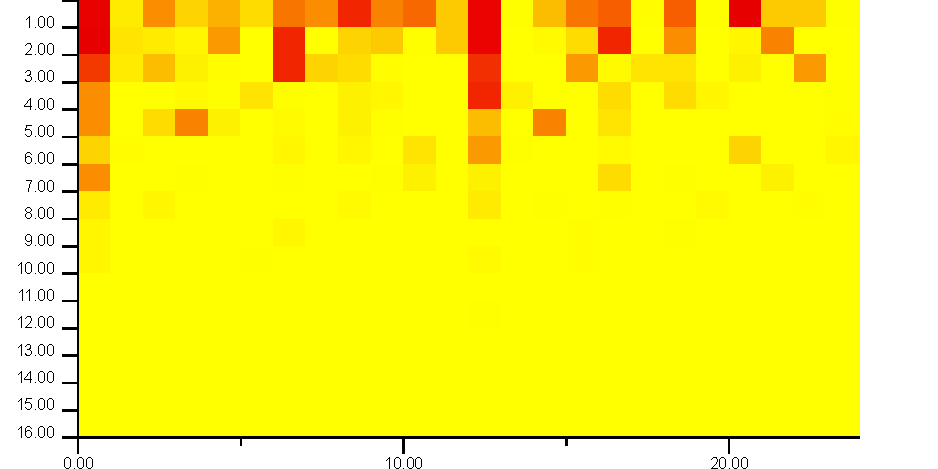
\includegraphics[width=1.0\textwidth]{./assets/hm-yellow-red.pdf}
\caption{Heat graph displaying note start points}
\label{fig:note-onset-hm}
\end{figure}

As you can see in the figure \ref{fig:note-onset-hm}, the majority of
activity is in the upper regions of the frequency spectrum and
concentrated at the beginning and the middle of the screen.

\begin{figure}[h]
\centering
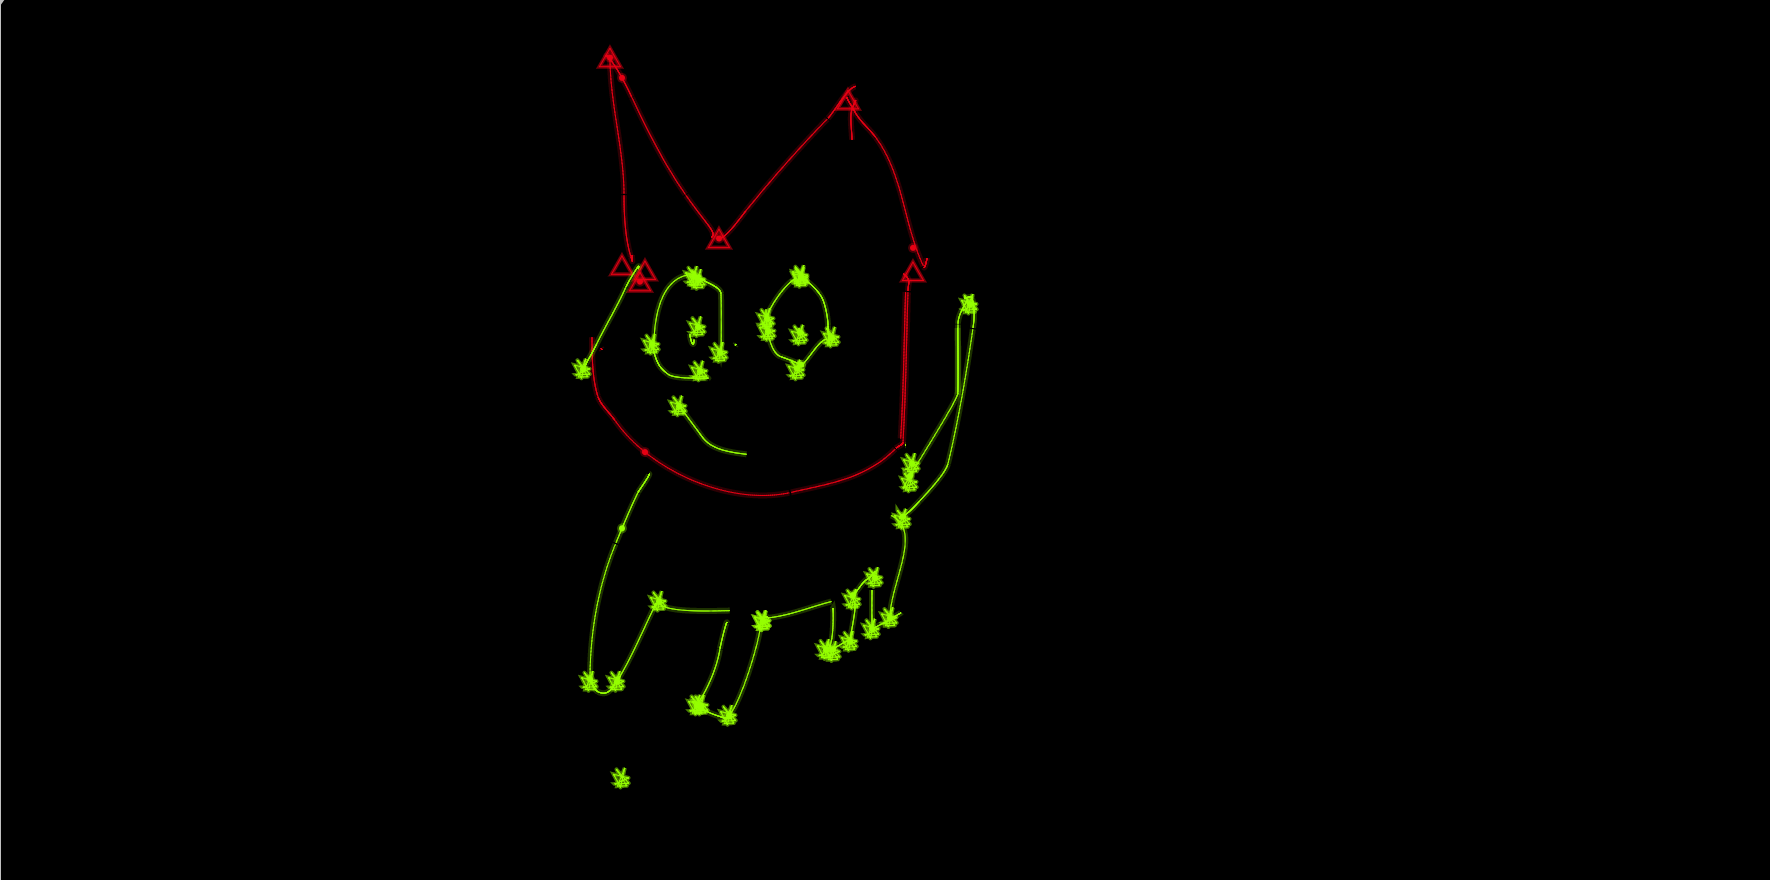
\includegraphics[width=1.0\textwidth]{./assets/exhibit-cat.png}
\caption{Some exhibit participants managed to draw figurative artwork!}
\label{fig:exhibit-cat}
\end{figure}

\pagebreak

\subsection{Performance issues}\label{performance-issues}

\subsection{Conclusion}\label{conclusion}

\end{document}
